\section{\label{sec:method}Methodology}
% MARK THIS NEEDS SOME ELABORATION

We ran multiple sets of \mc\ simulations to compare the directional performance of the various detector geometries.
Because we wanted to specifically focus on the inherent potential directionality of each approach, we determined \emph{not} to include backgrounds at this stage.
The idea here \dash particularly for the \santa\ design \dash was to investigate whether the (expected) improvement in directional capability offered sufficient reason to proceed to simulating and attempting to solve the (expected) difficulties with backgrounds.
Further details on each set are discussed below.

\subsection{\label{subsec:ncomp_params}Shared Parameters}

\begin{itemize}
  \item \textbf{Simulation \& Analysis software: RAT-PAC and ROOT}
  \item \textbf{10~000 IBD events were run in each detector}
  \item IBD events were separated in time by a Poisson distribution of mean 1~s
  \item In all cases but NuLat $3^3$, IBD vertices were distributed uniformly throughout the scintillator volume(s)
  \item No backgrounds for this portion of the study
  \begin{itemize}
    \item This allows each design's potential directional performance to manifest clearly
    \item Backgrounds are addressed in supplementary simulations %(see Ch.~\ref{ch:bgs}) 
  \end{itemize}
  \item Realistic position was simulated by either:
  \begin{itemize}
   \item Adding noise to raw MC data until reaching desired resolution, or
   \item Discretizing the relevant coordinate(s)
  \end{itemize}
  \item Remaining parameters are listed with respective results
\end{itemize}

\subsection{\label{subsec:esim}Early Simulations}

% params
\begin{table}[ht]
  \begin{tabular}{ c || c | c | c }
%   \hline
    % \textbf{~} & \textbf{\dc} & \textbf{\nl} & \textbf{\santa} \\ %\hline
    \textbf{~} & \textbf{DC} & \textbf{NL} & \textbf{SANTA} \\ %\hline
    % ~ & 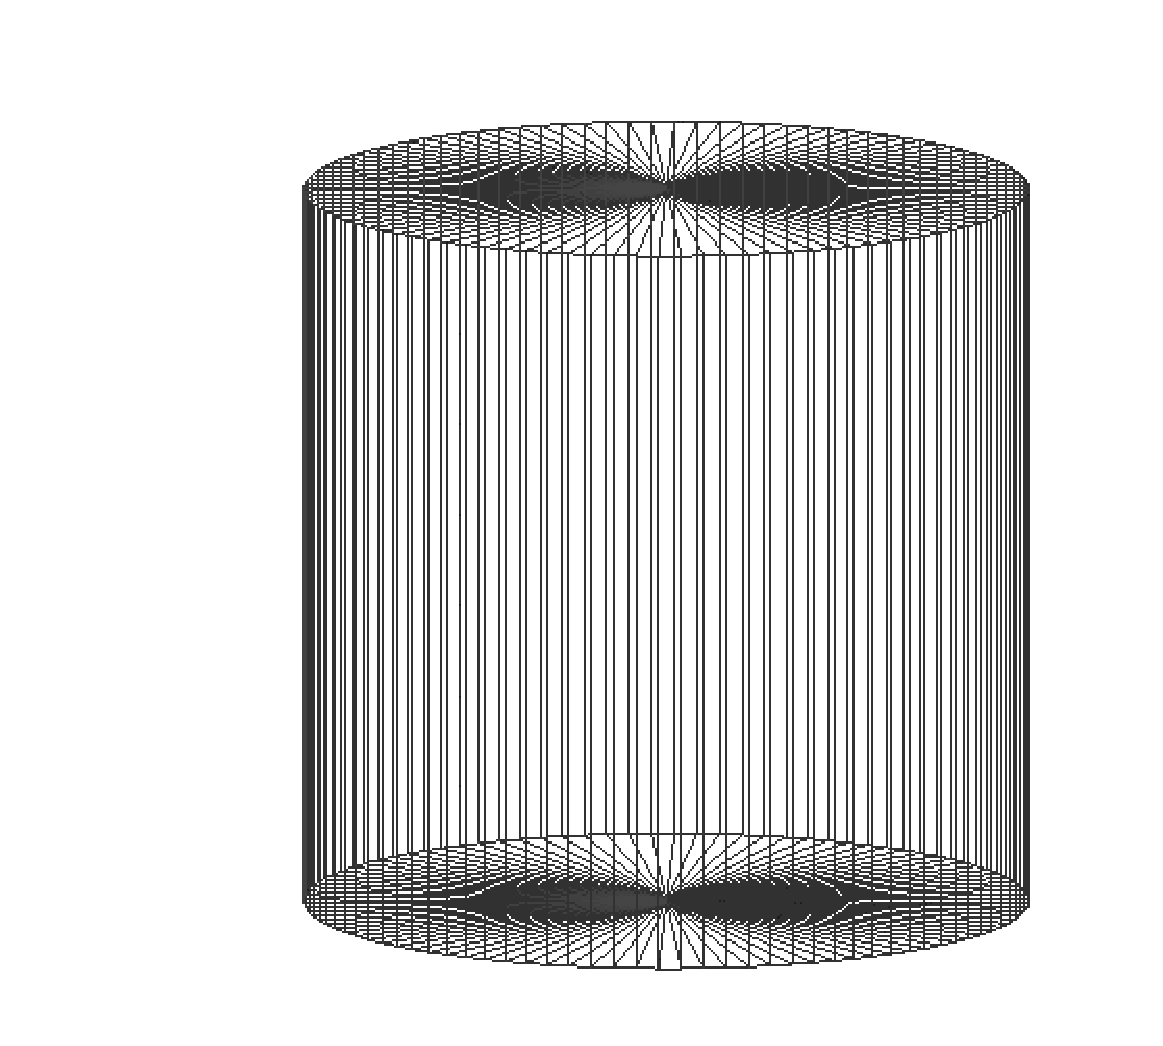
\includegraphics[width=0.2\linewidth]{figures/dc_geo_plain_white_gray.eps} & \
      % 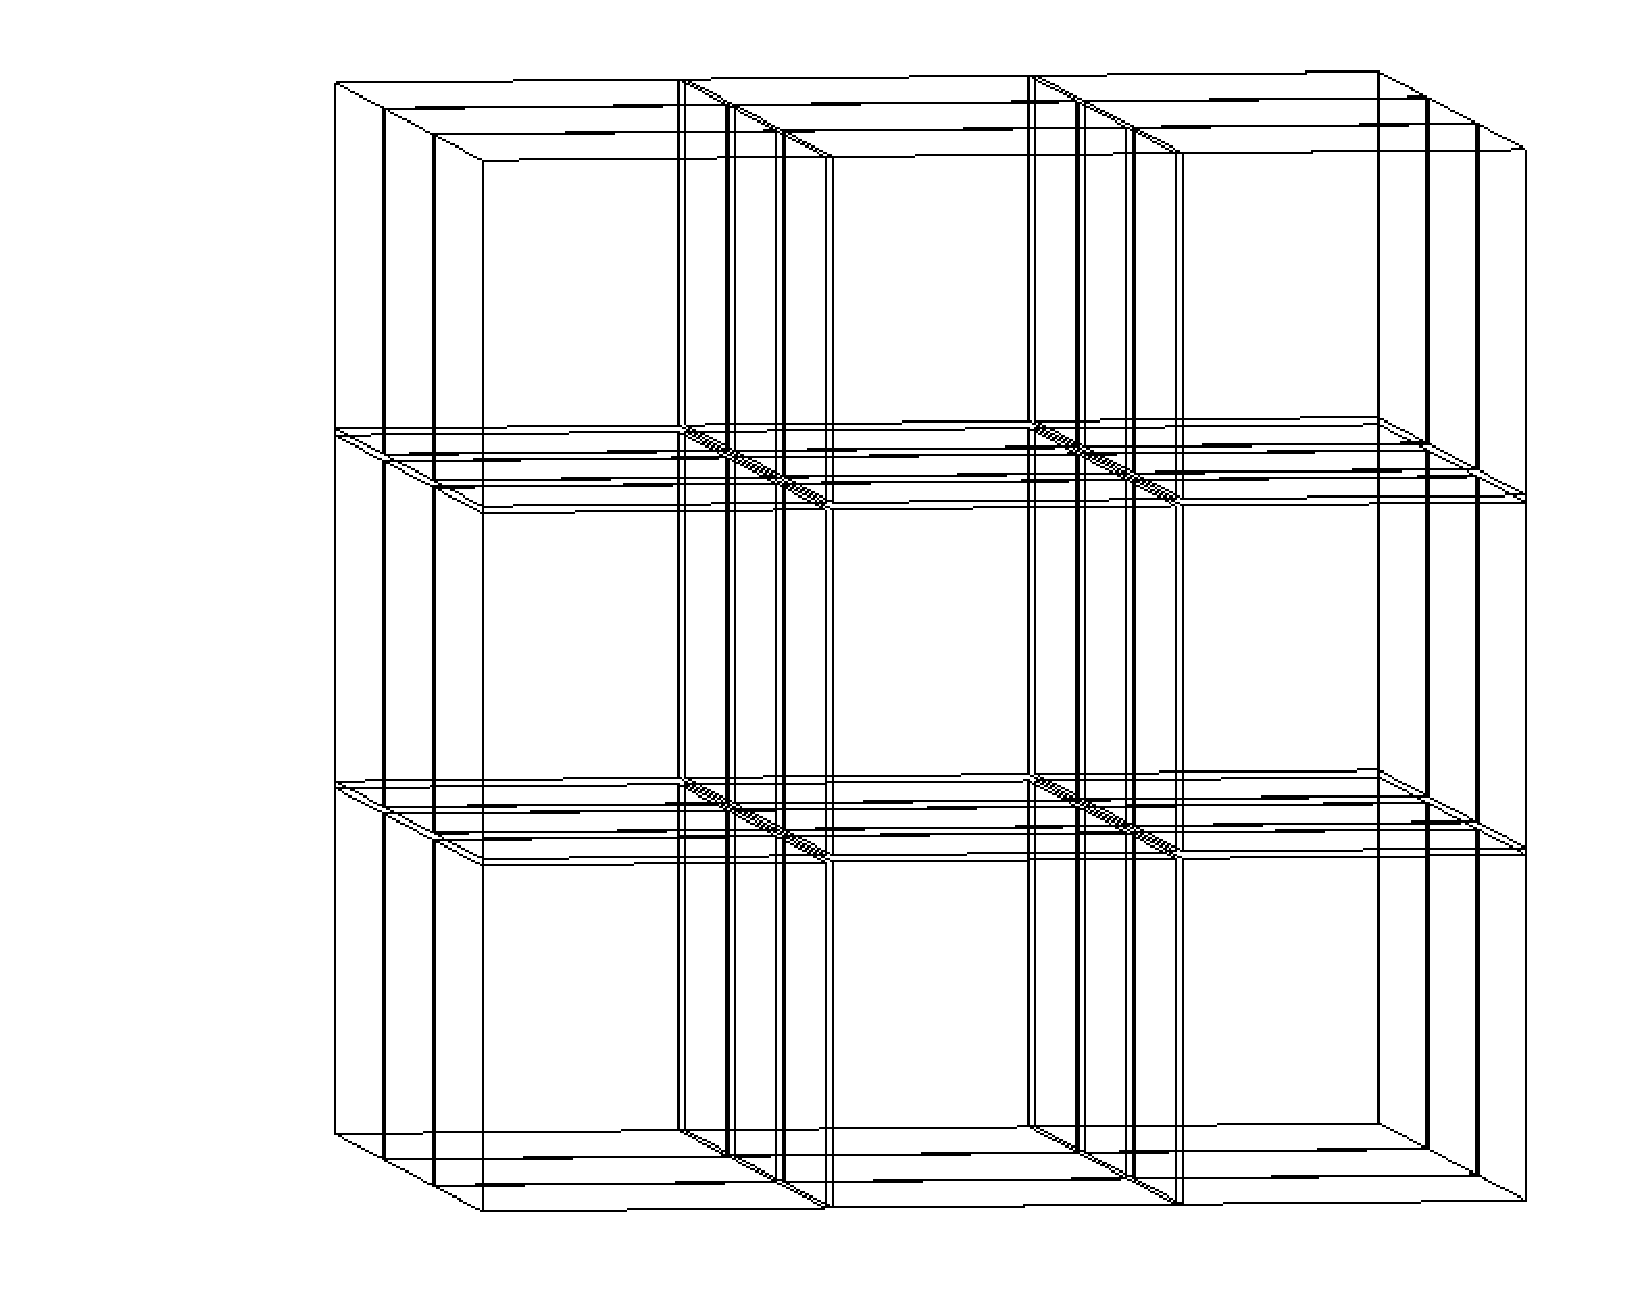
\includegraphics[width=0.2\linewidth]{figures/nl_geo_plain_white.eps} & \
      % 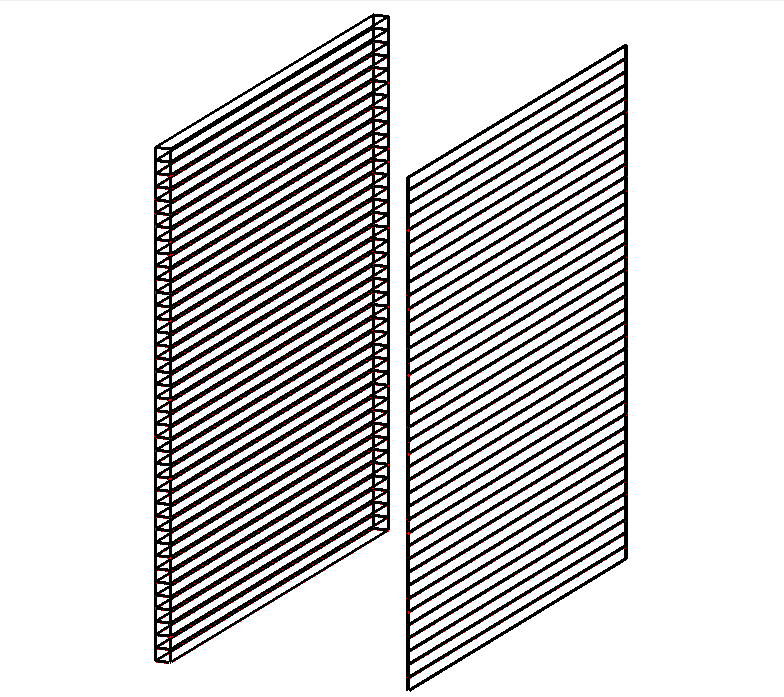
\includegraphics[width=0.2\linewidth]{figures/santa_plain3.png} \\ \hline \hline
    \hline \hline
    IBD~Volume(s) & target volume & central cube & target plane \\ \hline
    % Material & \dc\ \ols & EJ-254 & EJ-254 \\ \hline
    Material & DC LOS & EJ-254 & EJ-254 \\ \hline
    Doping & $\sim$0.1\%wt~natural~Gd & 1.5\%wt~$\nucl{6}{Li}$ & (0|1)\%wt~$\nucl{10}{B}$ \\
%   \hline
  \end{tabular}
  \caption{Summary of Simulation Parameters}
  \label{tab:comp_params}
\end{table}

We simulated 10~000 \ibd\ events in each of the following three experiments: \dc, \nl\ $3^3$, and \santa.
We took the \nb\ source to be distant enough that the incoming antineutrino flux could be well-represented by a plane wave; i.e., we took the incoming antineutrinos to be uniform in direction.
Furthermore, we took the \nb\ source to be located ``at the horizon'' relative to the detectors, normal to their side face(s).
For convenience, we placed our origins at the center of each detector with the $x$-axis pointing toward the \nb\ source, so that the incoming antineutrinos were traveling along $\{x,y,z\} = \{-1,0,0\}$.
The energy distribution for the \ibd\ events was taken from the built-in \rat\ reactor spectrum. %TODO: figure or citation here [cf. thesis] "(see \S\ref{subsec:basics_energy}, Fig.~\ref{fig:rp_ibd})."
The \ibd\ vertices were generated uniformly throughout a volume or set of volumes chosen specifically for each detector.
The target material for the \dc\ experiment was a \dc-style \ols\ doped at $\sim$~0.1\%wt~natural~Gd. Composition was carefully tuned in \rat\ to match the actual \dc\ target material as described in~\cite{2012JInst},~\cite{Caden:2012aap}.
The target material for the \nl\ experiment was Eljen 254 plastic scintillator doped at 1.5\%wt~$\nucl{6}{Li}$~\cite{Eljen}.
The target material for the \santa\ experiment was Eljen 254 plastic scintillator; the target plane was undoped, and the capture plane was doped at 5\%wt~natural~B (1\%wt~$\nucl{10}{B}$), as proposed in~\cite{Safdi:2014hwa}.
These parameters are summarized in Table~\ref{tab:comp_params}.

% results
\begin{table}[ht]
  \centering
  \newcolumntype{d}[1]{D{.}{.}{#1} }
  \begin{tabular}{ l || r | r | r | r }
    \textbf{Source} & \textbf{Total IBDs} & $\mathbf{N}$ & $\mathbf{\Delta\varphi\ (^o)}$ & $\mathbf{\Delta\varphi_{100}\ (^o)}$ \\
    \hline \hline
    DC (Data)~\cite{Caden:2012aap} & --- & 8~249 & 6~\, & --- \\ \hline
    DC (MC) & 10~000 & 10~000 & 6.9 & 77 \\ \hline
    NuLat (MC) & 10~000 & 5~423 & 2.3 & 15 \\ \hline
    SANTA (MC) & 10~000 & 3~232 & 0.4 & 1.9 \\
   \end{tabular}
  \caption{Summary of Comparative Results}
  \label{tab:comp_results}
\end{table}

% both sets of histograms
\begin{figure}[ht]
  \centering
  \begin{subfigure}{0.28\linewidth}
    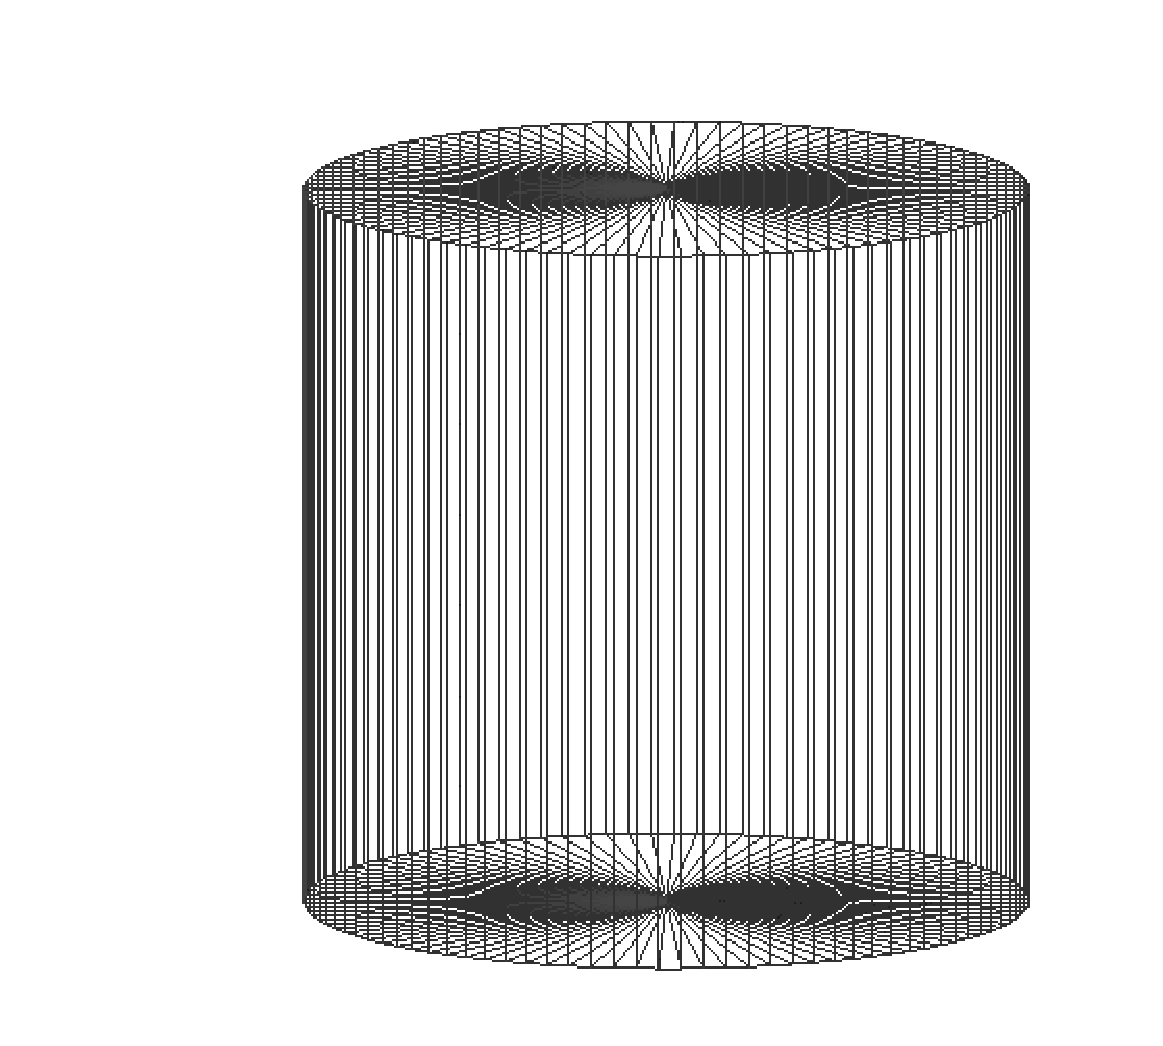
\includegraphics[width=1.0\linewidth]{figures/dc_geo_plain_white_gray.eps}
  \end{subfigure}
  \begin{subfigure}{0.28\linewidth}
    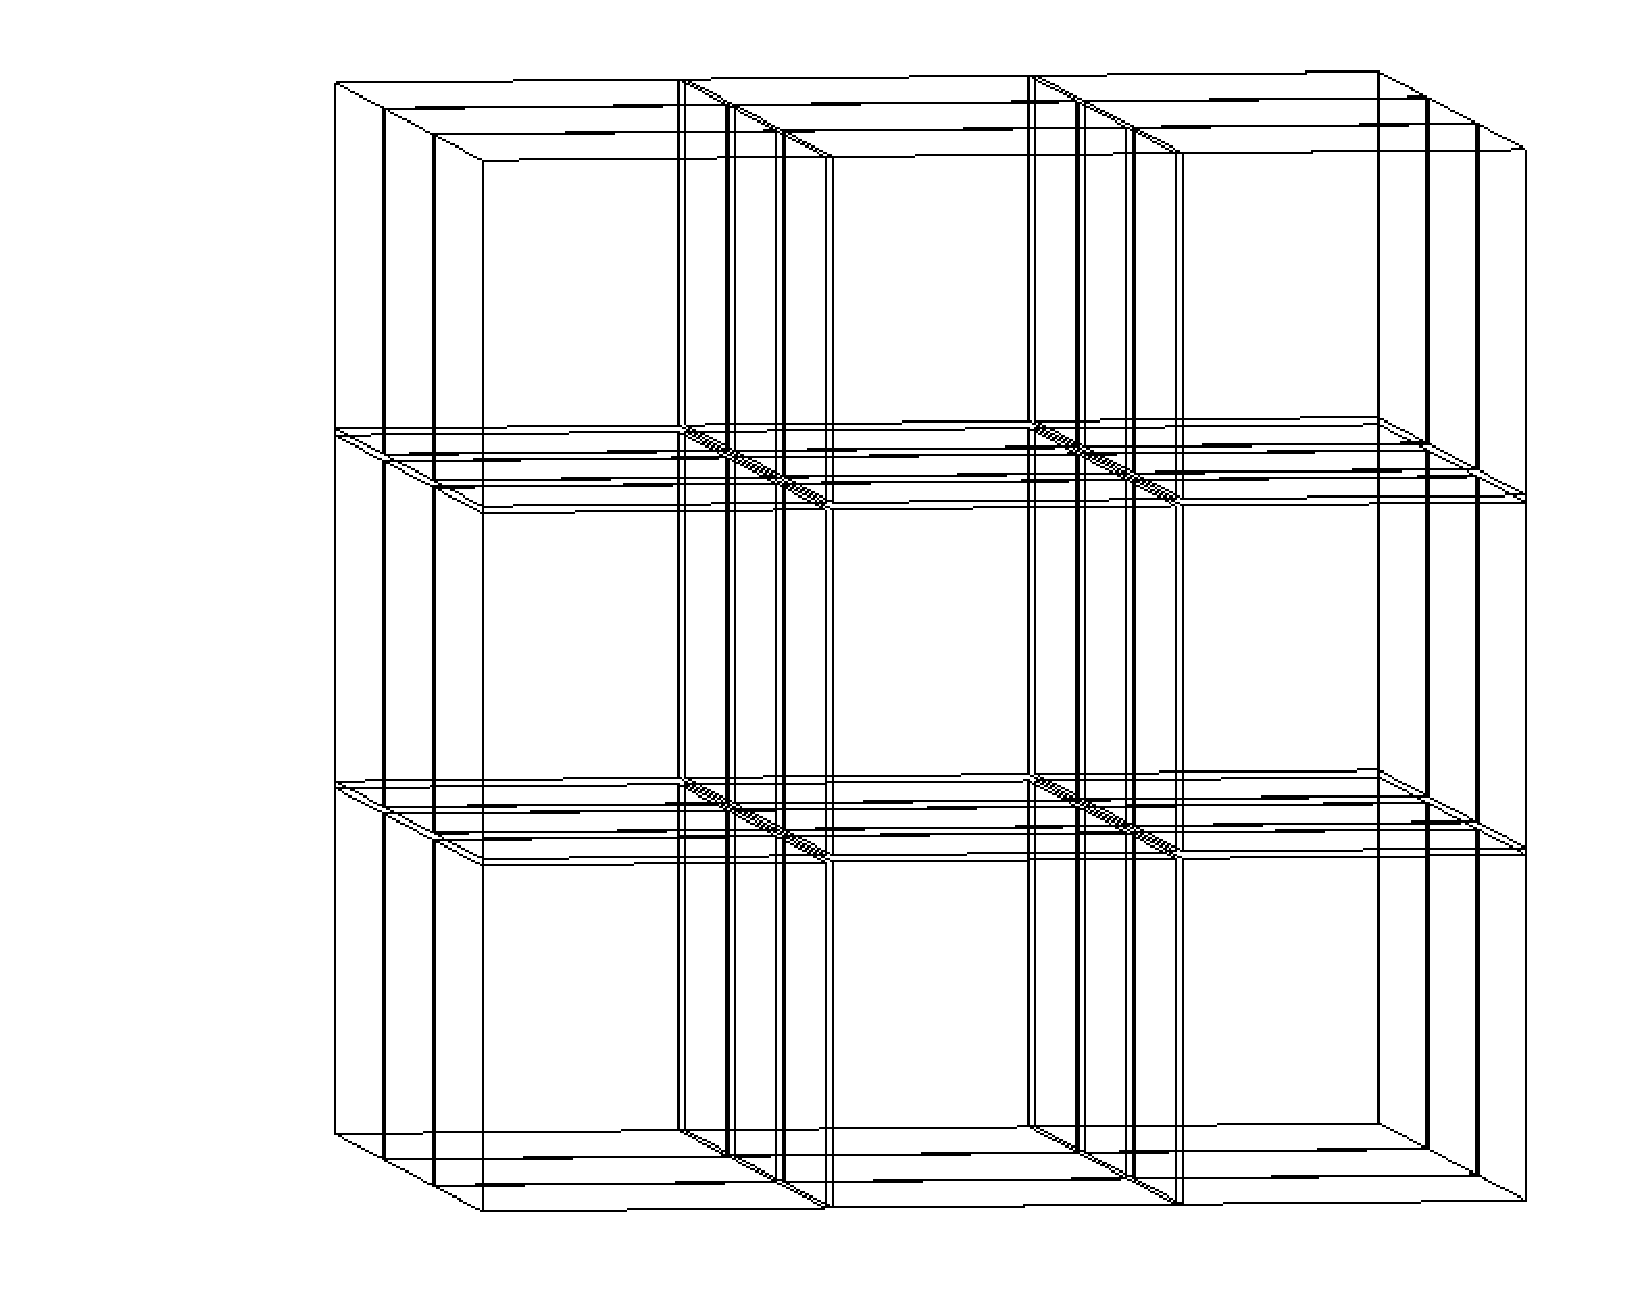
\includegraphics[width=1.0\linewidth]{figures/nl_geo_plain_white.eps}
  \end{subfigure}
  \begin{subfigure}{0.28\linewidth}
    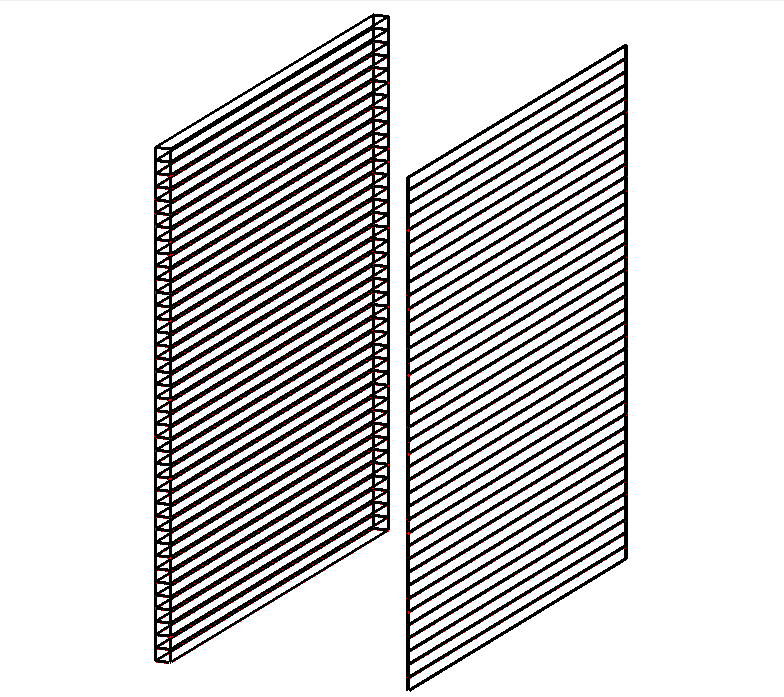
\includegraphics[width=1.0\linewidth]{figures/santa_plain3.png}
  \end{subfigure}\\
  \begin{subfigure}{0.8\linewidth}
    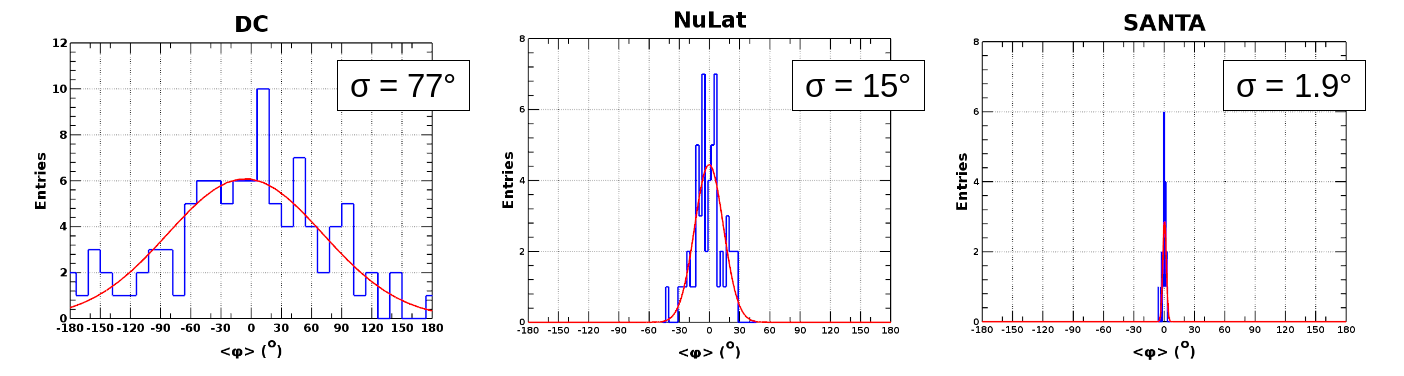
\includegraphics[width=1.0\linewidth]{figures/hund_phis.png}
  \end{subfigure}\\
  \begin{subfigure}{0.8\linewidth}
    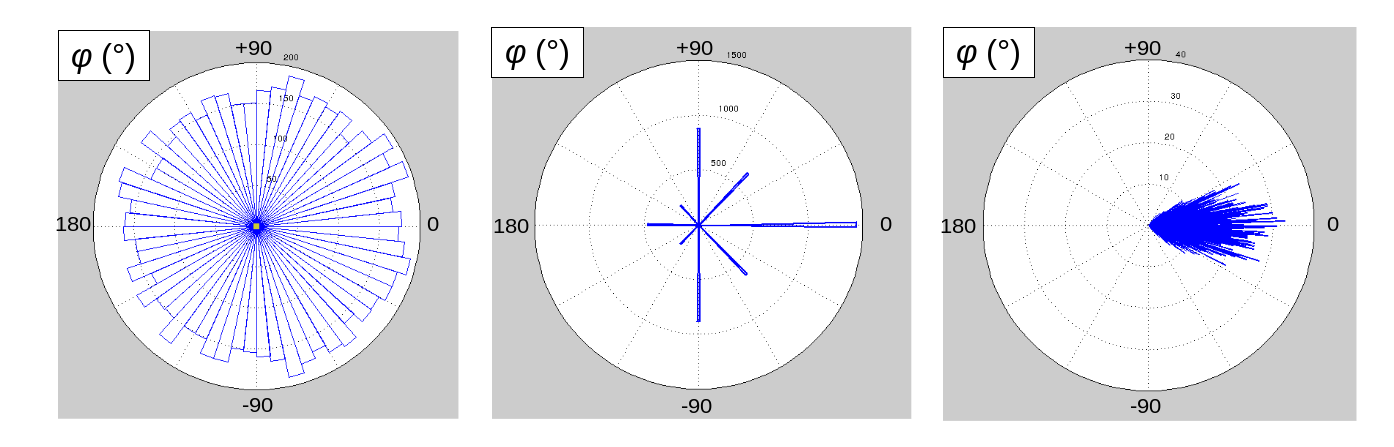
\includegraphics[width=1.0\linewidth]{figures/results_roses_only.png}
  \end{subfigure}
  \caption{Comparison of Directional Results}%: \
  \label{fig:comp_results}
\end{figure}

The full results of the (early) comparative simulations are given numerically in Table~\ref{tab:comp_results} and graphically in Fig.~\ref{fig:comp_results}.

\subsection{\label{subsec:nsim}New Simulations}

Building on the above simulations, we decided to run a new set of comparative simulations.
We added the new geometries described above*. %FIXME
We ran new simulations for the original geometries alongside the new ones, both to cross-check our results and to ensure that the final comparison would be as representative as possible. % bleh this sentence

During this process, we also developed the following upgrades to our analysis:
\begin{itemize}
  \item Migrated all non-ROOT analysis code to ROOT
  \item Streamlined and automated our simulation / analysis chain
  \item Developed software tools for analysis and visualization that we hope will be useful to the community in general and to \rat\ users in particular
\end{itemize}


\subsection{\label{subsec:bgs}Addressing Backgrounds}

\subsubsection{\label{subsubsec:bg_setup}Setup}

% How these detectors might behave in the presence of backgrounds is the obvious next question to ask.
How these detectors might behave in the presence of backgrounds is an obvious question to ask.
We have performed some work here as well, but it is important to properly contextualize.
The simulations presented in this work are not intended to provide full predictions of the detailed performance of these various experiments, but rather a first investigation of concepts and possible detector geometries.
Correspondingly, the primary purpose of adding backgrounds to these simulations is not to predict the detailed performance of fully-realized detectors, but rather to confirm that the results of the primary (i.e., IBD-only) simulations above are well-grounded by comparing our simulations against published data from an appropriate real-world detector.
To this end, we have chosen PROSPECT as our primary reference point, as it has well-characterized backgrounds and fits the low-overburden, near- to mid-field deployment scenario we are targeting.
We enclosed our simulated detector in a rectangular water shield extending 0.5~m outward from each exterior surface, as shown in Fig.~\ref{fig:bg_setup}. %TODO: Remake this figure with PROSPECT instead of NuLat

% BG configuration
\begin{figure}[ht]
  % \centering
  % \begin{subfigure}{0.45\linewidth}
  %   \includegraphics[width=\linewidth]{figures/santa_new.png}
  %   \caption{\santa}
  %   \label{subfig:bg_setup_santa}
  % \end{subfigure}
  % \begin{subfigure}{0.45\linewidth}
    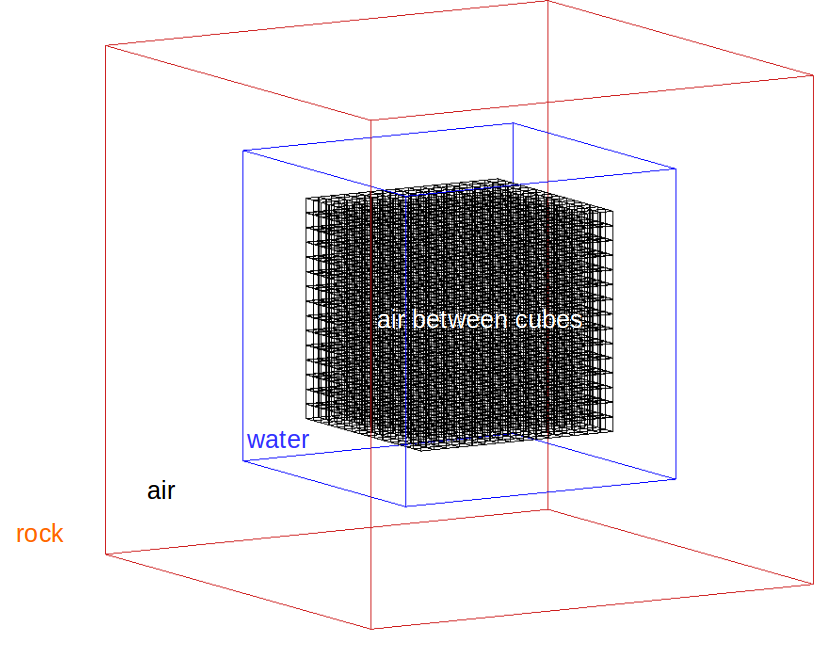
\includegraphics[width=\linewidth]{figures/nl_15.png}
    % \caption{$15^3$ \nl}
    % \label{subfig:bg_setup_nl}
  % \end{subfigure}
  % \caption{Configuration for Background Runs}
  \caption{Configuration for Background Runs, Using $15^3$ \nl\ as an Example}
  \label{fig:bg_setup}
\end{figure}

\subsubsection{\label{subsubsec:bg_sources}Sources}

% muogenic n0 spectrum
\begin{figure}
  \begin{center}
    
\includegraphics[width=1.0\linewidth]{figures/neutron_spectrum.png}
    \caption{Dominant Background: Muon-induced Fast Neutrons}
    \label{fig:bg_neutrons}
  \end{center}
\end{figure}

The dominant background in near-surface reactor-\nb\ experiments comes from fast neutrons induced by cosmogenic muons. These can scatter and/or capture in the target medium, producing a scintillation signal that can mimic a prompt or delayed event.
If the rates and/or energies are high enough, they can produce a complete signal pair that mimics an \ibd\ event.

The muogenic fast-neutron spectrum at sea level is shown in Fig.~\ref{fig:bg_neutrons}, created from data given in~\cite{2004ITNS51:3427G}.
This spectrum was integrated to get a total rate per $\mathrm{cm}^2$, then adjusted down to 1/7th the sea-level total to simulate $\sim$30~m.w.e. of overburden. % relative to reference standard mentioned above.
The resulting neutron flux per $\mathrm{cm}^{2}$ was then applied to the surfaces (walls, floor, ceiling) of the cave surrounding the detector, using neutron energies sampled randomly from the original spectrum. % resulting in the total rates given in Table~\ref{tab:bkgds_rates}.

\subsubsection{\label{subsubsec:bg_results}Background Results}

% prospect bgs by cut
\begin{figure}
  \begin{center}
    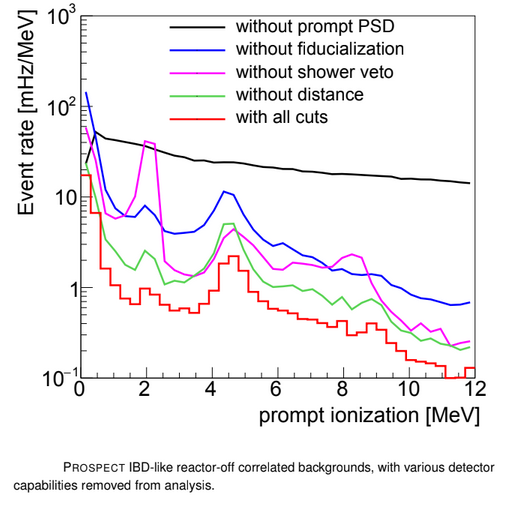
\includegraphics[width=0.7\linewidth]{figures/PROSPECT_bg_by_cut.png}
    %\caption{PROSPECT Backgrounds by Cut~\cite{Mendenhall:2018}}
    \caption{PROSPECT Backgrounds by Cut~\cite{Mendenhall:2018}\\ \textit{Note: ``PSD'' = Pulse-Shape Discrimination}}
    \label{fig:bgs_prospect}
  \end{center}
\end{figure}

% results table
\begin{table}[ht]
  \centering
  \begin{tabular}{c|c|c}
    Quantity & Rate (Hz) & Rate (day$^{-1}$)\\ \hline
    $R_S$ & 1.0 & 90~000\\
    $R_P$ & 0.48 & 41~500\\
    $^{R_S}/_{R_P}$ & $\bm{2.17}$ & $\bm{2.17}$
  \end{tabular}
  \caption{Background-Comparison Results}
  \label{tab:bg_results}
\end{table}

Our quantity for comparison is the rate of false-positive IBD events:
\begin{itemize}
  \item caused by muogenic fast-neutrons (either scatter-capture or coincident capture-capture),
  \item that are tagged by the neutrino trigger,
  \item subjected to the same cuts.
\end{itemize}
We will denote this quantity as $R_S$ and $R_P$ for our simulated rate and the actual PROSPECT rate, respectively.
We have estimated $R_P$ from the published PROSPECT plot (\emph{black line}) shown in Fig.~\ref{fig:bgs_prospect}~\cite{Mendenhall:2018}.
Given the base level of detail appropriate to our work, we have selected a factor of 3 as our rough indicator of agreement.
In other words, we posit that if $R_S$ falls within a factor of 3 of $R_P$, then our simulations are behaving reliably.
The results are shown in Table~\ref{tab:bg_results}.


\subsubsection{\label{subsubsec:selection}Detector Selection}

\begin{table*}[ht]
  %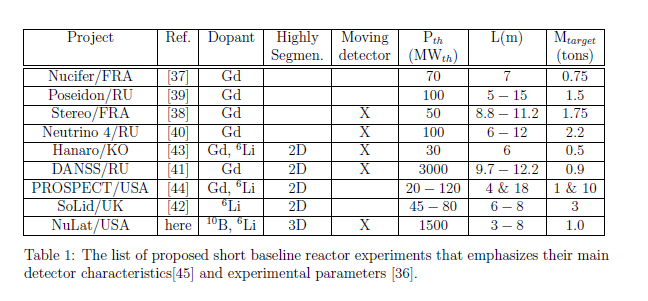
\includegraphics[width=0.6\linewidth]{figures/sbre.png}
  %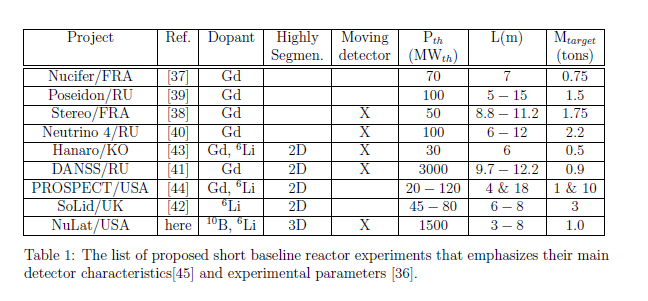
\includegraphics[width=0.9\linewidth]{figures/sbre.png}
  %\caption[2015 Summary of Short-Baseline Reactor-Antineutrino Experiments]{2015 Summary of Short-Baseline Reactor-Antineutrino Experiments}



\begin{tabular}{|c|c|c|c|c|c|c|}
\hline
Project       & Dopant             & \begin{tabular}[c]{@{}c@{}}Highly\\ Segmen.\end{tabular} & \begin{tabular}[c]{@{}c@{}}Moving \\ Detector\end{tabular} & \begin{tabular}[c]{@{}c@{}}P$_{th}$\\ (MW$_{th})$\end{tabular} & \begin{tabular}[c]{@{}c@{}}L\\ (m)\end{tabular} & \begin{tabular}[c]{@{}c@{}}M$_{target}$\\ (tons)\end{tabular} \\ \hline
Nucifer/FRA   & Gd                 &                                                          &                                                            & 70                                                             & 7                                               & 0.75                                                          \\ \hline
Poiseidon/RU  & Gd                 &                                                          &                                                            & 100                                                            & 5-15                                            & 1.5                                                           \\ \hline
Stereo/FRA    & Gd                 &                                                          & X                                                          & 50                                                             & 8.8-11.2                                        & 1.75                                                          \\ \hline
Neutrino 4/RU & Gd                 &                                                          & X                                                          & 100                                                            & 6-12                                            & 2.2                                                           \\ \hline
Hanaro/KO     & Gd, $^{6}$Li       & 2D                                                       & X                                                          & 30                                                             & 6                                               & 0.5                                                           \\ \hline
DANSS/RU      & Gd                 & 2D                                                       & X                                                          & 3000                                                           & 9.7-12.2                                        & 0.9                                                           \\ \hline
PROSPECT/USA  & Gd, $^{6}$Li       & 2D                                                       &                                                            & 20-120                                                         & 4 \& 18                                         & 1 \& 10                                                       \\ \hline
SoLid/UK      & $^{6}$Li           & 2D                                                       &                                                            & 45-80                                                          & 6-8                                             & 3                                                             \\ \hline
NuLat/USA     & $^{10}$B, $^{6}$Li & 3D                                                       & X                                                          & 1500                                                           & 3-8                                             & 1.0                                                           \\ \hline
\end{tabular}



  
  \caption[2015 Summary of Short-Baseline Reactor-Antineutrino Experiments]{2015 Summary of Short-Baseline Reactor-Antineutrino Experiments ~\cite{Lane:2015alq}.\\ 
  %\textit{Note: The table number and reference numbers appearing within this reproduction refer to the original paper~\cite{Lane:2015alq} and not to this document.}
  }
  \label{tab:sbre}
\end{table*}

Now that we have described each of the experiments we chose to simulate, we would like to briefly discuss why we selected this particular collection.

There are a number of experiments we could have chosen to represent each fundamental detector type.
%The field in general is well-represented in the 2015 survey of planned short-baseline reactor-antineutrino experiments shown in Table~\ref{tab:sbre}, reproduced from~\cite{Lane:2015alq}\footnote{Note that the table number and reference numbers appearing within this reproduction refer to the original paper~\cite{Lane:2015alq} and not to this dissertation.}. %FIXME: footnotes not supported by this document class
The field in general is well-represented in the 2015 survey of planned short-baseline reactor-antineutrino experiments shown in Table~\ref{tab:sbre}, reproduced from~\cite{Lane:2015alq}. %FIXME: footnotes not supported by this document class
Most of the detectors in the table were designed for a simple measurement of the neutrino flux and not for neutrino directionality.
As a result, our examination of one or two designs from each type \dash monolithic / non-highly-segmented (\dc), 2D-segmented (PROSPECT, \sandd), and 3D-segmented (\nl) \dash covers the field of short-baseline reactor experiments as far as antineutrino directionality is concerned.

Numerous factors were involved in selecting the particular detectors we used to represent their respective design types.
% Because I personally worked on the \mtc, \nl, and \sandd\ experiments, and my dissertation committee includes members of these collaborations as well as \dc\ and PROSPECT, these detectors were naturally optimal choices for use in this study.
Because members of our group personally worked on the \mtc, \nl, and \sandd\ experiments, and our faculty includes members of the \dc\ and PROSPECT collaborations, these detectors were naturally optimal choices for use in this study.
The \santa\ design is the only one of its type, so its inclusion was essentially predetermined.
Finally, the checkerboard and other hybrid designs appear here because they were developed by our group as a part of this work.



